\subsection{Mismatched Crowdsourcing}
\label{s6:mc}

\begin{figure}
  \centerline{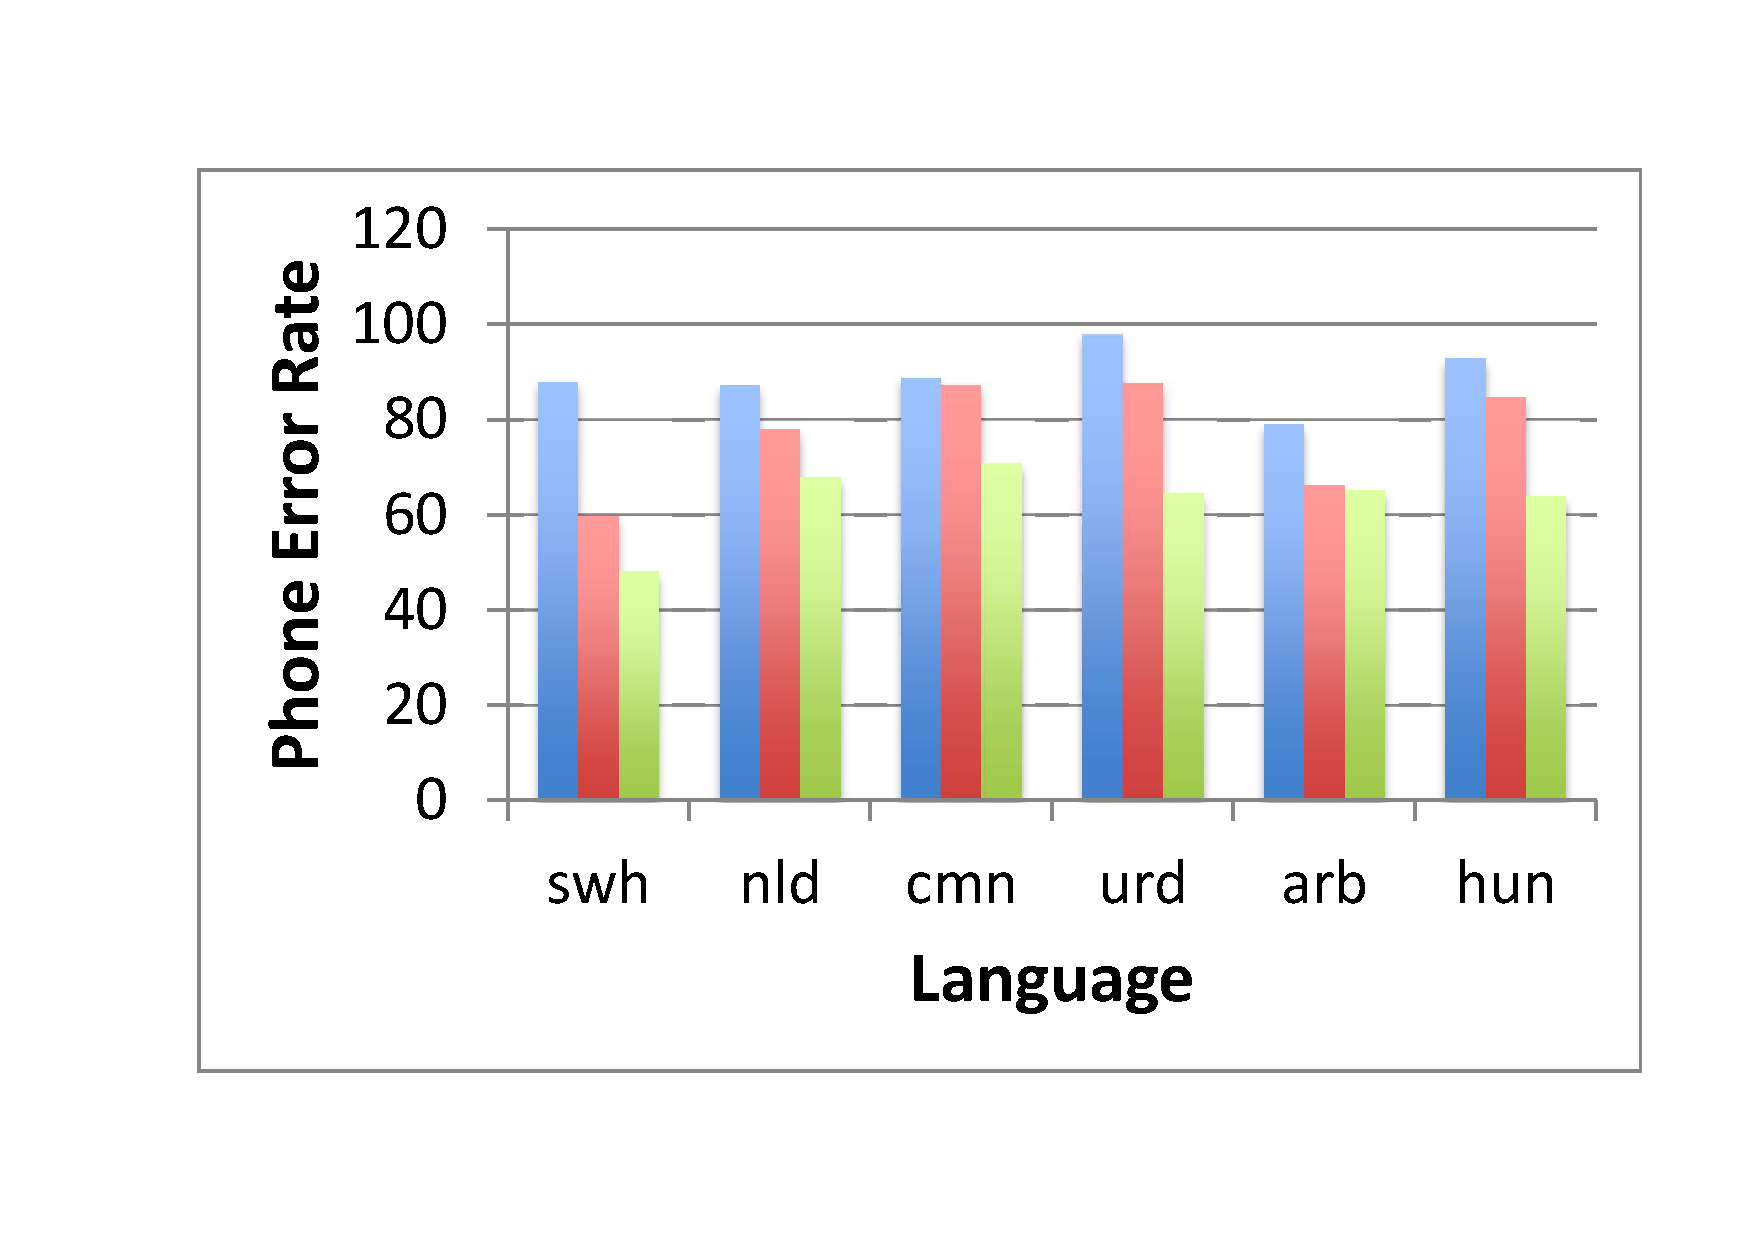
\includegraphics[width=4in]{../figs/lm_results.pdf}}
  \caption{PER of the 1-best path: a measure of the quality of
    probabilistic transcriptions acquired from mismatched
    crowdsourcing.  Native transcriptions were available in six
    languages: Swahili (swh), Dutch (nld), Mandarin (cmn), Urdu (urd),
    Arabic (arb), and Hungarian (hun).  Probabilistic transcriptions
    were decoded using three different methods per language: using a
    universal phoneme set (tallest bar in each language), using a
    phoneme set specific to the target language (middle bar in each
    language), and using a phonotactic language model derived from
    Wikipedia texts (shortest bar in each language).}
  \label{fig:pt_decode_per}
\end{figure}
%% KC: caption should not reference "tallest bar" etc, but rather should
%% refer to colors.

The quality of a probabilistic transcription derived from mismatched
crowdsourcing is significantly improved by using a phone language
model during the decoding process ($\rho(\phi)$ in Eq.~\ref{eq:PT}).
A crude measure of the quality of the PTs is given by the phone error
rate between $\phi^* = \argmax_{\phi} \rho(\phi|T)$ and the reference
phone sequences, called the ``label phone error rate'' (LPER). Phone
language models for each target language were computed from Wikipedia
texts using the methods described in Sec.~\ref{sec:trainwithlm}.
LPER of the 1-best path through the resulting PTs are shown in
Fig.~\ref{fig:pt_decode_per}.  As shown, the use of a phonotactic
language model, derived from Wikipedia text, reduces PER by about 10\%
absolute, in each language.

%\begin{table}[t]
%\centering
%\begin{tabular}{|c||c|c|c|c|c|c|c|}
%  \hline
%  & \multicolumn{7}{|c|}{Language (ISO 639-3 Code)}\\ \hline
%& arb & yue & nld & hun & cmn & swh & urd \\ \hline\hline
%Dev set (1-best PER) & 65.8 & 66.4 & 68.9 & 63.7 & 70.9 & 47.6 & 67.2 \\
%Eval set (1-best PER) & 66.2 & 67.8 & 70.9 & 63.5 & 69.6 & 50.3 & 70.5 \\\hline
%\end{tabular}
%\caption{Error rates (PER) of probabilistic transcripts computed from
%  mismatched crowdsourcing (non-native human listeners): Phone error
%  rate (PER) of the 1-best path through the probabilistic
%  transcription, $\phi^*=\argmax\rho(\phi|T)$, development and
%  evaluation sets.}
%\label{tab:LPER}
%\end{table}

%Table~\ref{tab:LPER} lists LPERs on the development and evaluation
%sets, for all seven languages.
LPER of the 1-best path does not
accurately reflect the extent of information in the PTs that can be
leveraged during ASR adaptation.  Consider, for example, the four
Urdu phones~\ipa{[p,p\textsuperscript{h},b,\"*b]}.  An attentive
English-speaking transcriber must choose between the two letters
$<$p,b$>$ in order to represent any of these four phones.  The
misperception G2P therefore maps the letters $<$p,b$>$ into a
distribution over the phones~\ipa{[p,p\textsuperscript{h},b,\"*b]}.
There is no reason to expect that the maximizer of
$\rho(\phi|\lambda)$ is correct, but there is good reason to expect
the correct answer to be a member of a short $N$-best list ($N\le 4$
phones/grapheme).  A fuller picture is therefore obtained by
considering a collection of sequences $\phi$ that are almost as
probable as $\phi^*$ according to our model. Figure~\ref{fig:listPER}
shows the trend of phone error rates (for three languages) obtained by
using collections $\phi$ of increasing size, plotted against an
entropy estimate of $\phi$, e.g., 1 bit of entropy allows two equally
probable choices for each phone in $\phi$. We note that the phone
error rates significantly drop across all languages, staying within 1
bit of entropy per phone, illustrating the extent of information
captured by the PTs.

\begin{figure}[t!]
\begin{center}
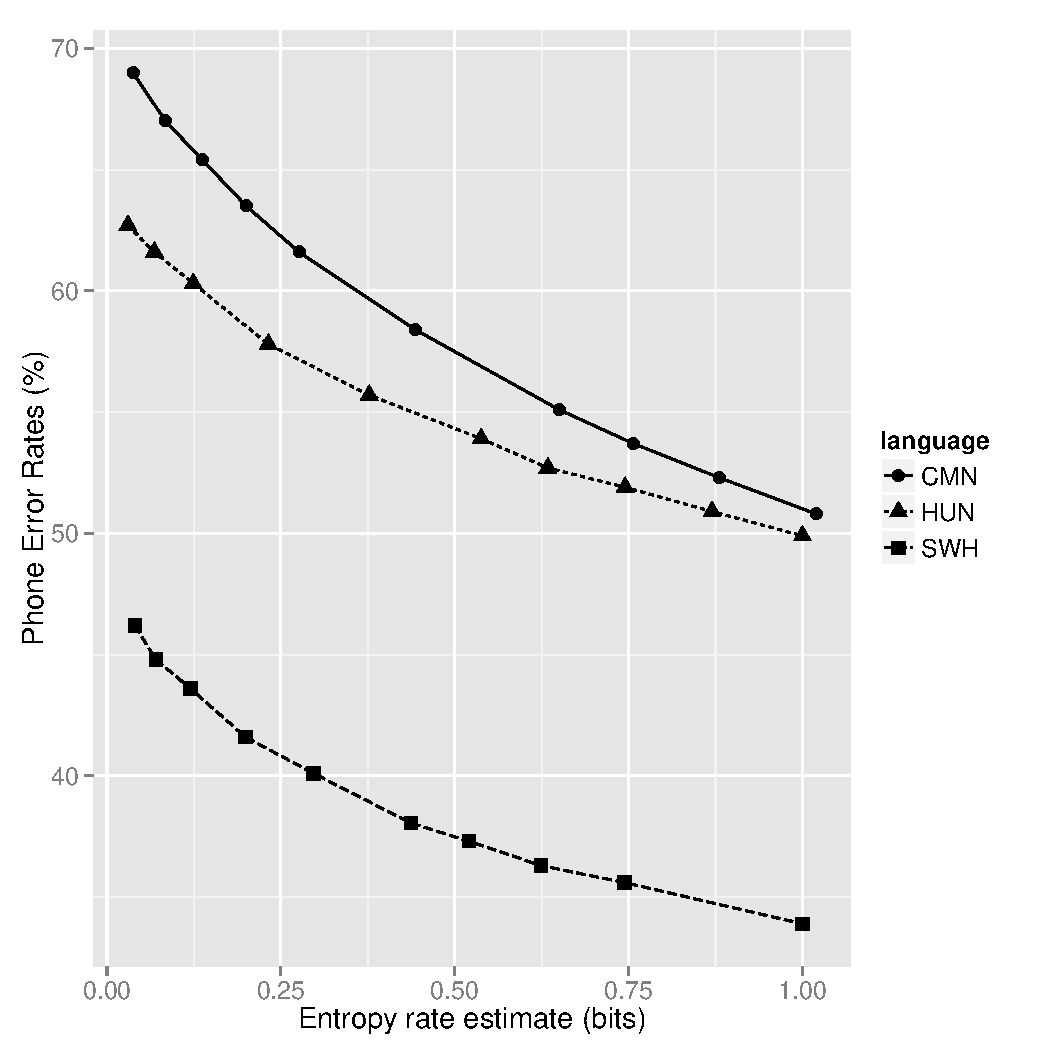
\includegraphics[width=3in]{../figs/perfig.pdf}
\end{center}
\caption{LPER plotted against entropy rate estimates of phone sequences in three different languages.}
\label{fig:listPER}
\end{figure}

